%!TEX root = ../Demo.tex
\chapter{引言}
不用看了,本文内容其实和章名没多大关系,只是没得名起了,迎合《本科生毕业设计(论文)工作手册》要求而已。

\section{文字处理}

\subsection{字体设置}
\textbf{\kaishu {西安电子科技大学}}(Xidian University)简称“\textbf{西电}”或“\textbf{西军电}”,坐落于古都西安。学校是中央部属高校,教育部直属、工信部共建,国家首批“{\heiti 211工程}”,是“{\fangsong 985工程优势学科创新平台}”、“111计划”、“2011计划”重点建设高校{ (中国电子信息领域、邮电领域唯一的“2011计划”牵头高校)},35所示范性软件学院的高校之一、集成电路人才培养基地的高校之一,56所获批设立研究生院的重点大学之一,也是{\zihao{-3} 北京高科大学联盟}的重要成员。 

1931年1月28日,红一方面军{ 总司令朱德、总政委毛泽东}于小布总部签发“调学生学无线电的命令”,随后,第一期无线电训练班在\CJKunderline{小布镇陈家土楼}正式开课。后迁移至\CJKunderdblline{瑞金},成立\CJKunderwave{中央军委无线电学校},是毛泽东等老一辈革命家亲手创建的第一所工程技术学校。1958年学校迁址西安,1966年转为地方建制,1988年定为西安电子科技大学。该校是中国最早建立\CJKunderdot{信息论、信息系统工程、雷达、微波天线、电子机械、电子对抗}等专业的高校之一,开辟了中国IT学科的先河,形成了鲜明的电子与信息学科特色与优势。毛泽东曾先后两次为该校题词:“\textbf{\large 全心全意为人民服务}”、“\textbf{\large 艰苦朴素}”。\footnote{从百度百科粘下来的,就不放进参考文献了。}

\CJKsout{来点没用的}

\subsection{数字转中文}
 测试数字:1234.233. 转为中文数字:\zhnumber{1234.233};转为中文字符串:\zhdigits{1234.233}。

\section{表格}

\subsection{普通表格}
先来看一个无标题的普通表格:

\begin{tabular}{|c|c|c|}
\hline
标题 & 标题 & 标题\\
\hline
1 & 2 & 3\\
\hline
\end{tabular}

如果想要居中可以使用 \verb=center= 环境。

带标题表格。
\begin{table}[ht]
\centering
\caption{普通表格1}\label{Tab:table1}
\begin{tabular}{L{2cm}C{2cm}R{2cm}}
\hline
标题 & 标题 & 标题\\
\hline
1 & 2 & 3\\
\hline
\end{tabular}
\end{table}

来一个表格并排,每个表格一个标题:
\begin{table}[ht]
\centering
\begin{minipage}{.45\textwidth}
\centering
\caption{并排表格1}\label{Tab:table1-1}
\begin{tabular}{lcr}
\hline
标题 & 标题 & 标题\\
\hline
1 & 2 & 3\\
\hline
\end{tabular}
\end{minipage}
\begin{minipage}{.45\textwidth}
\centering
\caption{并排表格2}\label{Tab:table1-2}
\begin{tabular}{lcr}
\hline
标题 & 标题 & 标题\\
\hline
1 & 2 & 3\\
\hline
\end{tabular}
\end{minipage}
\end{table}

再来一个表格并排
\begin{table}[ht]
\centering
\caption{并排表格}
\subcaptionbox{并排表格1}
{
\begin{tabular}{lcr}
\hline
标题 & 标题 & 标题\\
\hline
1 & 2 & 3\\
\hline
\end{tabular}
}
\subcaptionbox{并排表格2}
{
\begin{tabular}{lcr}
\hline
标题 & 标题 & 标题\\
\hline
1 & 2 & 3\\
\hline
\end{tabular}
}
\end{table}


\subsection{复杂点的表格}
表 \ref{Tab:table2} 主要用到的是列合并单元格、跨行合并单元格、混合合并单元格、表格横线的自定义粗细以及控制表格横线的自定义连接等。\footnote{表格虽然难看,主要是为了让大家看效果,里面技巧选用。}
\begin{table}[ht]
\centering
\caption{复杂表格}\label{Tab:table2}
\begin{tabular}{|c|c|c|c|}
\toprule[1pt]
\multicolumn{2}{|c|}{1} & 3 & 4\\
\midrule[0.5pt]
5 & 6 & 7 & \multirow{2}*{8}\\
\cline{1-3}
9 & 10 & 11 & \\
\midrule[0.5pt]
\multicolumn{2}{|c|}{\multirow{2}*{13}} & 15 & 16\\
\cline{3-4}
\multicolumn{2}{|c|}{} & 19 & 20\\
\bottomrule[1pt]
\end{tabular}
\end{table}

下面是另外一个长表格

为了在某些情况下方便的展示状态之间的关系,也把状态转移图写成表格,如图中的自动机,写成表格\ref{tab:sample}:
\begin{table}[!htbp]
    \caption{状态转移函数}
    \label{tab:sample}
    \centering
    \footnotesize% fontsize
    \setlength{\tabcolsep}{4pt}% column separation
    \renewcommand{\arraystretch}{1.2}%row space 
    \begin{tabular}{cccccc} 
        \hline 
        %\multirow{2}{*}{状态说明} & \multirow{2}{*}{状态} & \multicolumn{4}{c}{输入字符} \\
        \multirow{2}*{状态说明}      &    \multirow{2}*{状态}    & \multicolumn{4}{c}{输入字符} \\
                                    &   &$a$ & $b$ & $1$ & $\epsilon$ \\
        \hline
        开始状态(start)  & $q_0$ & -     & $q_1$  &      - &     -    \\
                        & $q_1$ & $q_2$ &    -   &    -   &    $q_2$ \\
        结束状态(accept) & $q_2$ &   -   & -      & $q_2$  &    -     \\
        \hline 
    \end{tabular}
\end{table}

表格填充颜色,如表 \ref{Tab:table3} 所示。此次,主要用到的出上述介绍外,有单个单元格填充颜色、整列填充颜色、整行填充颜色;此外,还添加了单元格划分的功能。

\begin{table}[ht]
\centering
\caption{填色表格}\label{Tab:table3}
\begin{tabular}{c | c| >{\columncolor{yellow}}c}
\toprule[1pt]
\diagbox{No.}{Title} & \textbf{L-Title} & \textbf{R-Title}\\
\hline
\rowcolor{red} 1 & One & First\\
\cellcolor[rgb]{.9,.9,.9} 2 & Two & Second\\
\cellcolor[rgb]{.2,.9,.9} 3 & Three & Third\\
\bottomrule[1pt]
\end{tabular}
\end{table}

以上,就是普通表格的常用例子了,其他的应用技巧以及功能大家自学吧,毕竟这只是个模板的使用样例,不是\LaTeX{} 教案。
\subsection{长表格}

呐,在开始长表格之前,我们应该怎么样呢?对,先说点废话。为什么呢?你想啊,既然是长表格,肯定是能够跨页存在的,不说点废话把它顶下去,顶到换页,咋能对得起它的NB功能呢,是吧。

咳咳,严肃点,主角登场了。表 \ref{Tab:longtable} 就是这一小节的主角——长表格了。首先说明一下,这种表格如果放的数据太多的话,就不要在正文里面用了,放到附录里就可以了。

\begin{longtable}[c]{cC{2cm}C{2cm}C{2cm}C{2cm}}
\caption{这是一个长表格}\label{Tab:longtable}\\
\hline
行号 & 标题1 & 标题2 & 标题3 & 标题4\\
\hline
\endfirsthead %以上是最前的表头
\multicolumn{5}{c}{\zihao{5}续表 \thetable\quad 这是一个长表格}\\
\hline
行号 & 标题1 & 标题2 & 标题3 & 标题4\\
\hline
\endhead %以上是换页后的表头,如未换页,并不会显示
\hline
\multicolumn{5}{r}{接下页续表……}\\
\endfoot %以上是前页的表尾,如未换页,并不会显示。
\hline
\endlastfoot%以上选填最后也的表尾。一般不填
%下面开始长表格的内容
1 & 1 & 2 & 3 & 4\\
2 & 5 & 6 & 7 & 8\\
3 & 9 & 10 & 11 & 12\\
4 & 13 & 14 & 15 & 16\\
5 & 17 & 18 & 19 & 20\\
6 & 21 & 22 & 23 & 24\\
7 & 25 & 26 & 27 & 28\\
8 & 29 & 30 & 31 & 32\\
9 & 33 & 34 & 35 & 36\\
10 & 37 & 38 & 39 & 40\\
11 & 41 & 42 & 43 & 44\\
12 & 45 & 46 & 47 & 48\\
13 & 49 & 50 & 51 & 52\\
14 & 52 & 54 & 55 & 56\\
15 & 57 & 58 & 59 & 60\\
16 & 61 & 62 & 63 & 64\\
17 & 65 & 66 & 67 & 68\\
18 & 69 & 70 & 71 & 72\\
19 & 73 & 74 & 75 & 76\\
20 & 77 & 78 & 79 & 80\\
21 & 81 & 82 & 83 & 84\\
22 & 85 & 86 & 87 & 88\\
23 & 89 & 90 & 91 & 92\\
24 & 93 & 94 & 95 & 96\\
25 & 97 & 98 & 99 & 100\\
\end{longtable}



\section{图片}
\subsection{普通图片的插入}
如同表格一样,插图一般都用浮动体来控制,这样排出来的文章美观。\footnote{本文涉及到的所有图片,除我校校徽等标记外,均为个人拍摄。}比如,图 \ref{Fig:xd1} 所示,是一个图片的样例。
\begin{figure}[ht]
  \centering
  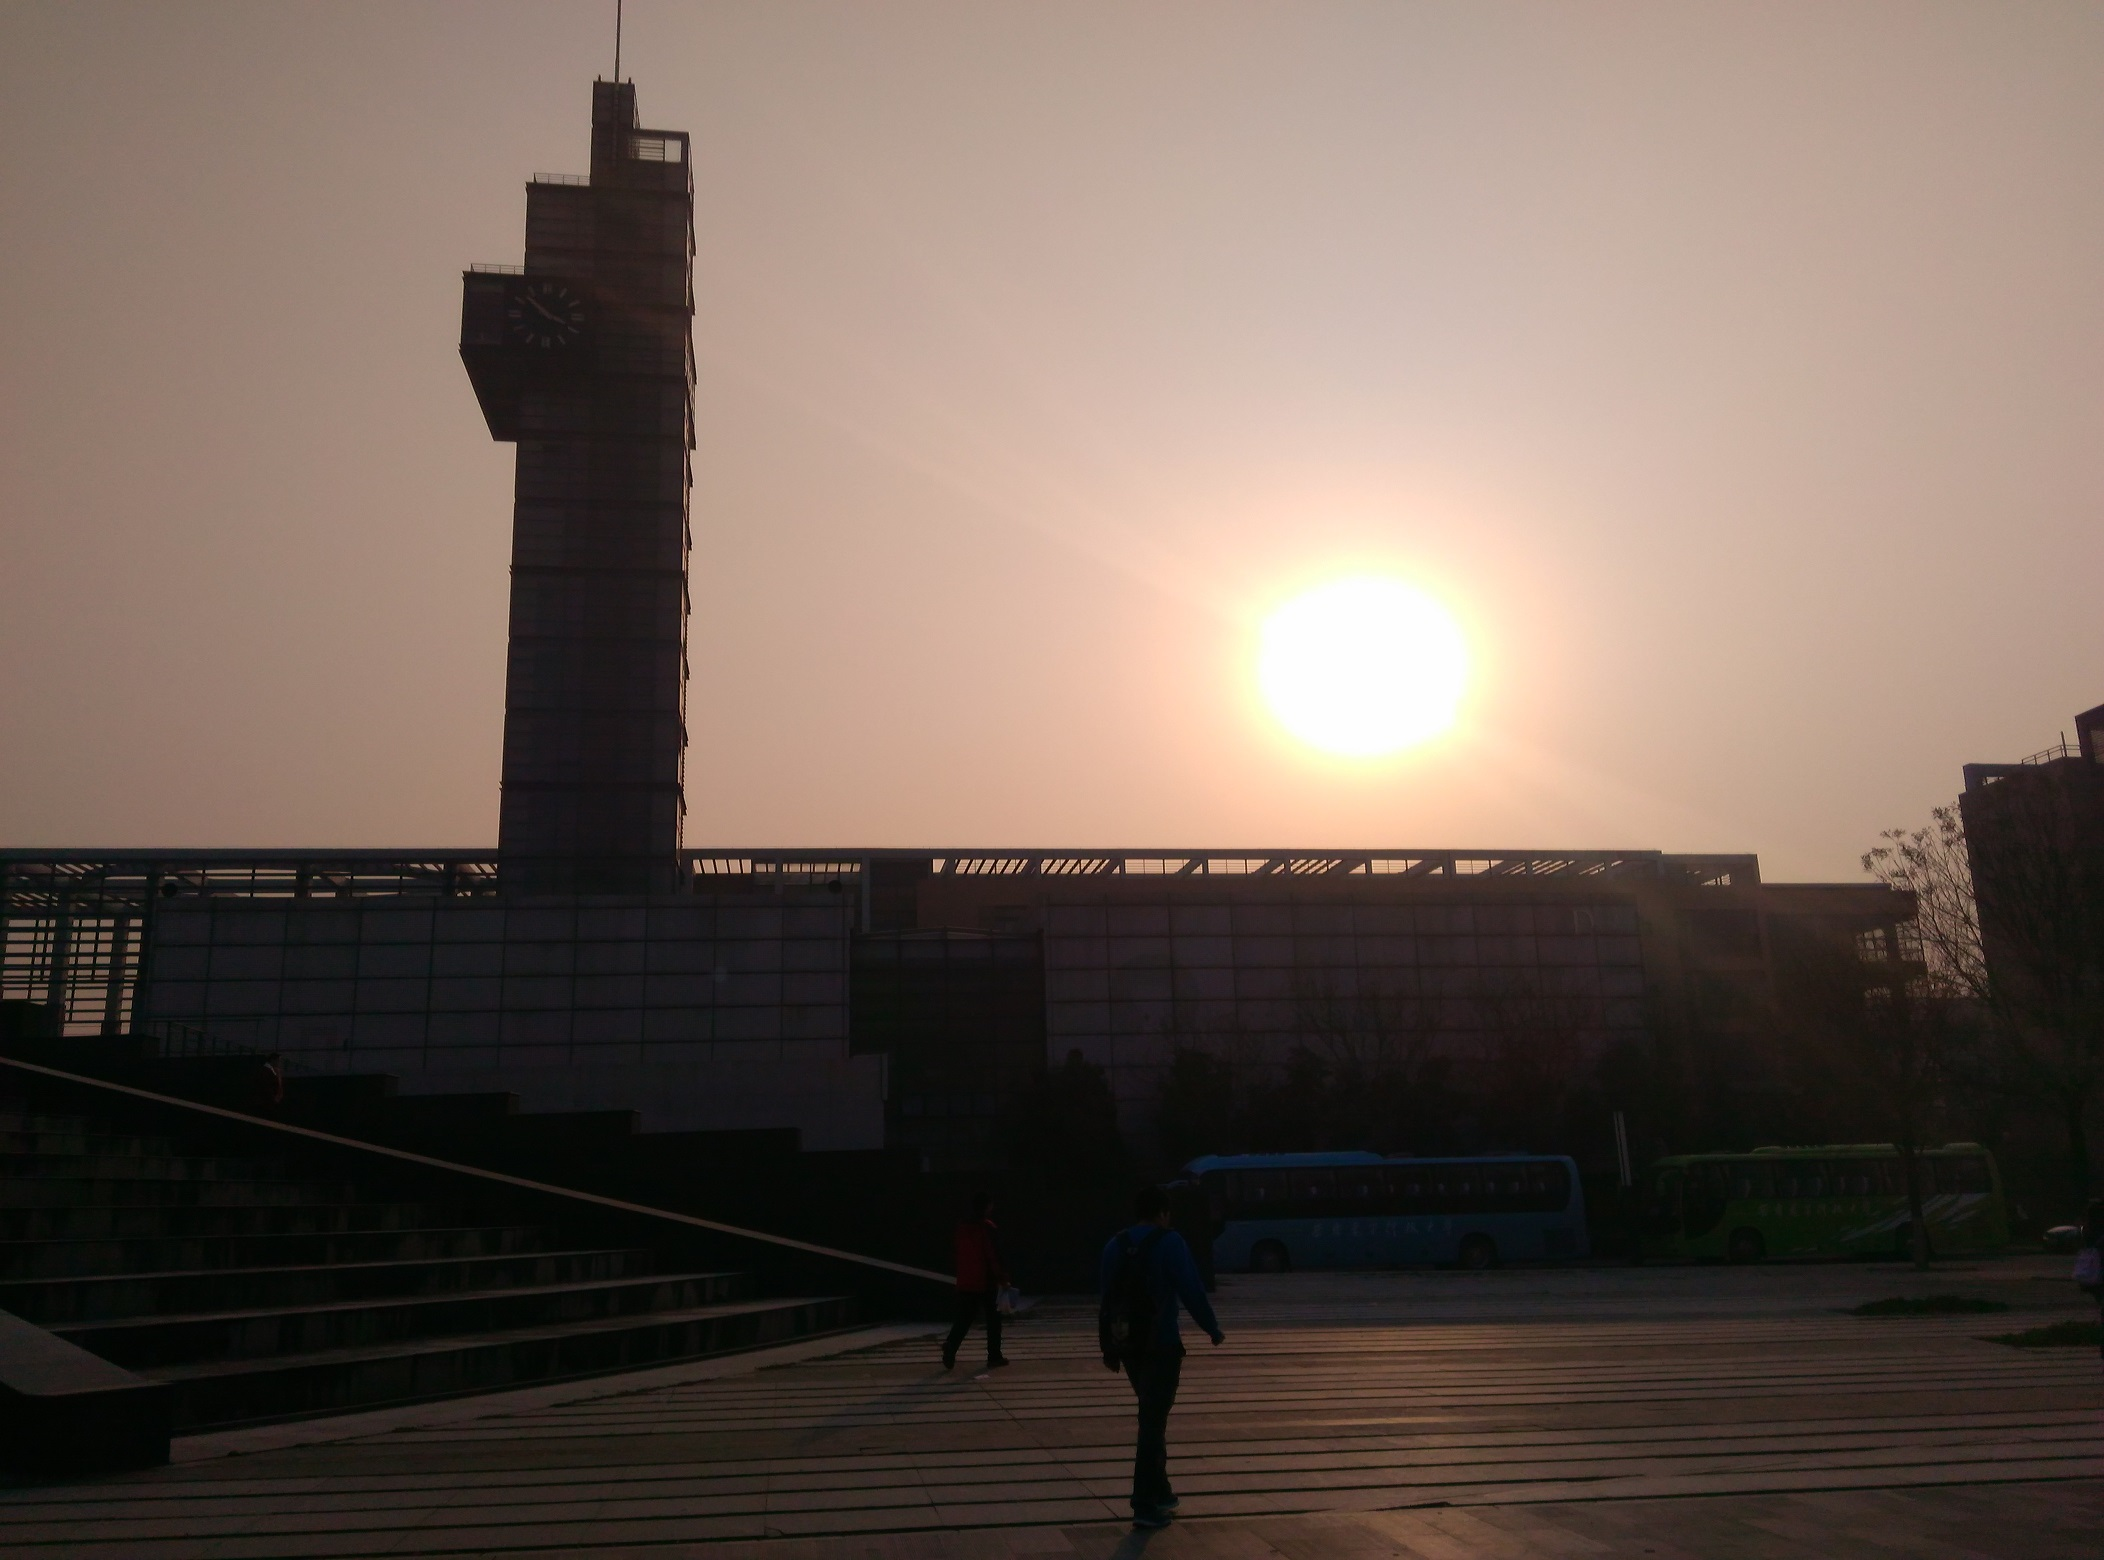
\includegraphics[width=0.8\linewidth]{./Figure/IMG_XD1.jpg}
  \caption{西电1}\label{Fig:xd1}
\end{figure}

\subsection{图片并排插入}

先来看第一个,两个图片分别一个标题,如图 \ref{Fig:xd2} 和 图 \ref{Fig:xd3}.
\begin{figure}[ht]
\centering
\begin{minipage}{.45\textwidth}
\centering
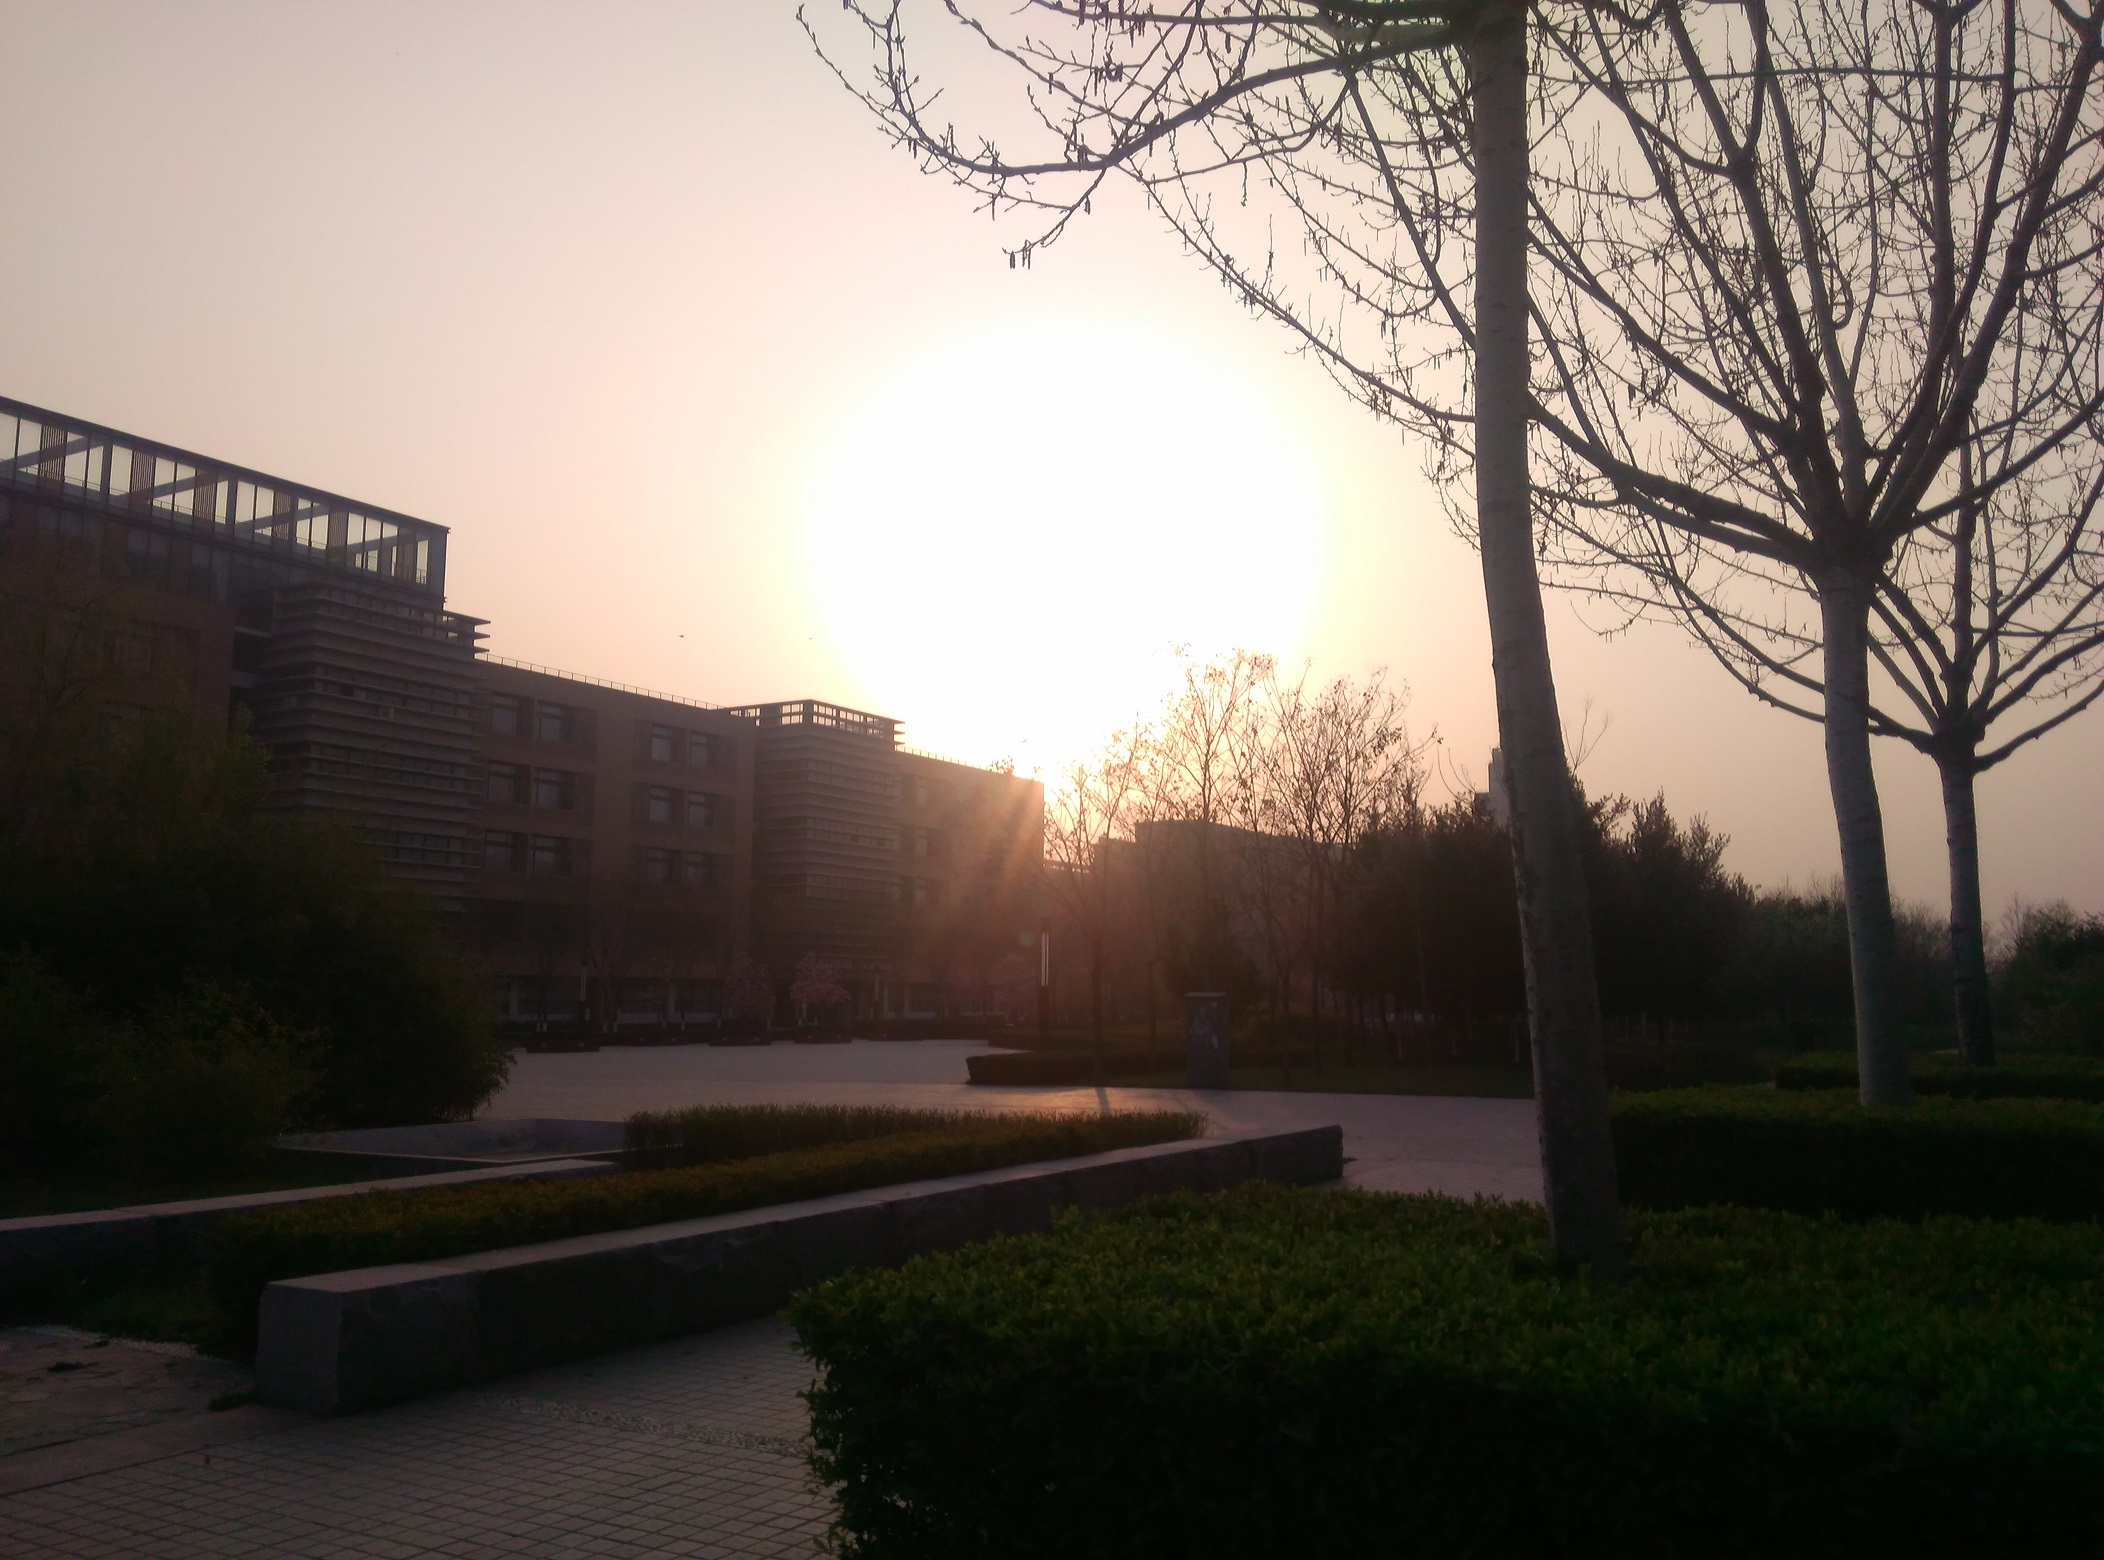
\includegraphics[width=1\linewidth]{./Figure/IMG_XD2.jpg}
  \caption{西电2}\label{Fig:xd2}
\end{minipage}~
\begin{minipage}{.45\textwidth}
\centering
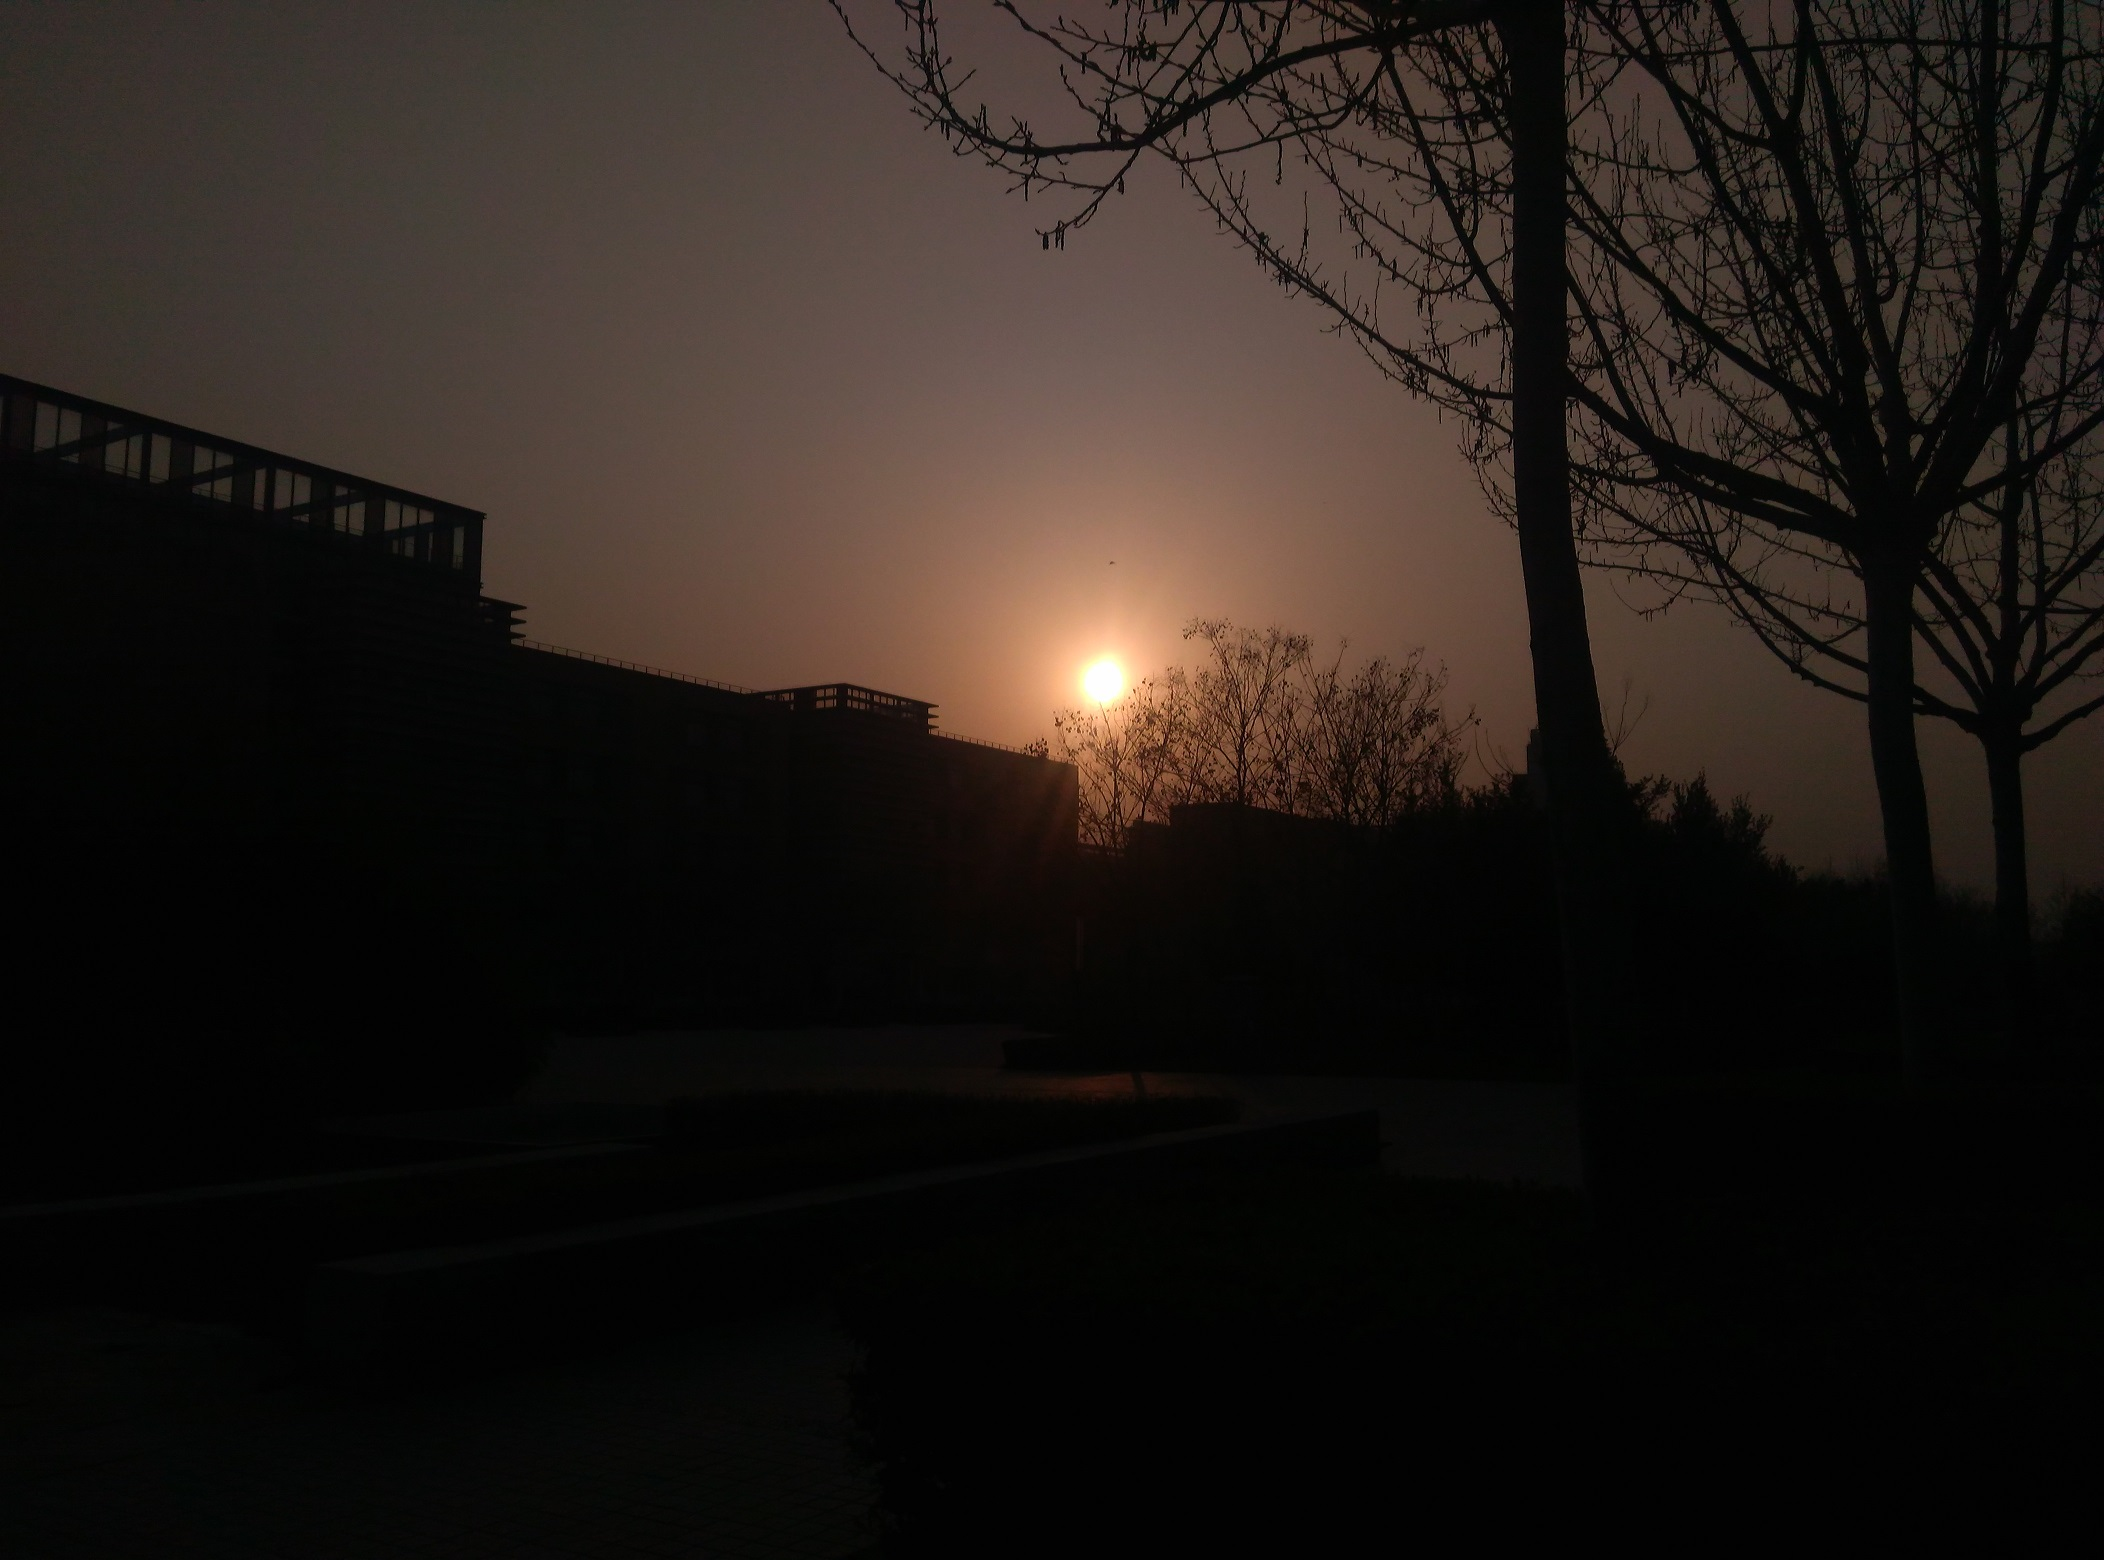
\includegraphics[width=1\linewidth]{./Figure/IMG_XD3.jpg}
  \caption{西电3}\label{Fig:xd3}
\end{minipage}
\end{figure}

再来看一个统一大标题带子标题的,如图 \ref{Fig:bingpai} 所示。
\begin{figure}[ht]
\centering
\subcaptionbox{西电4}
{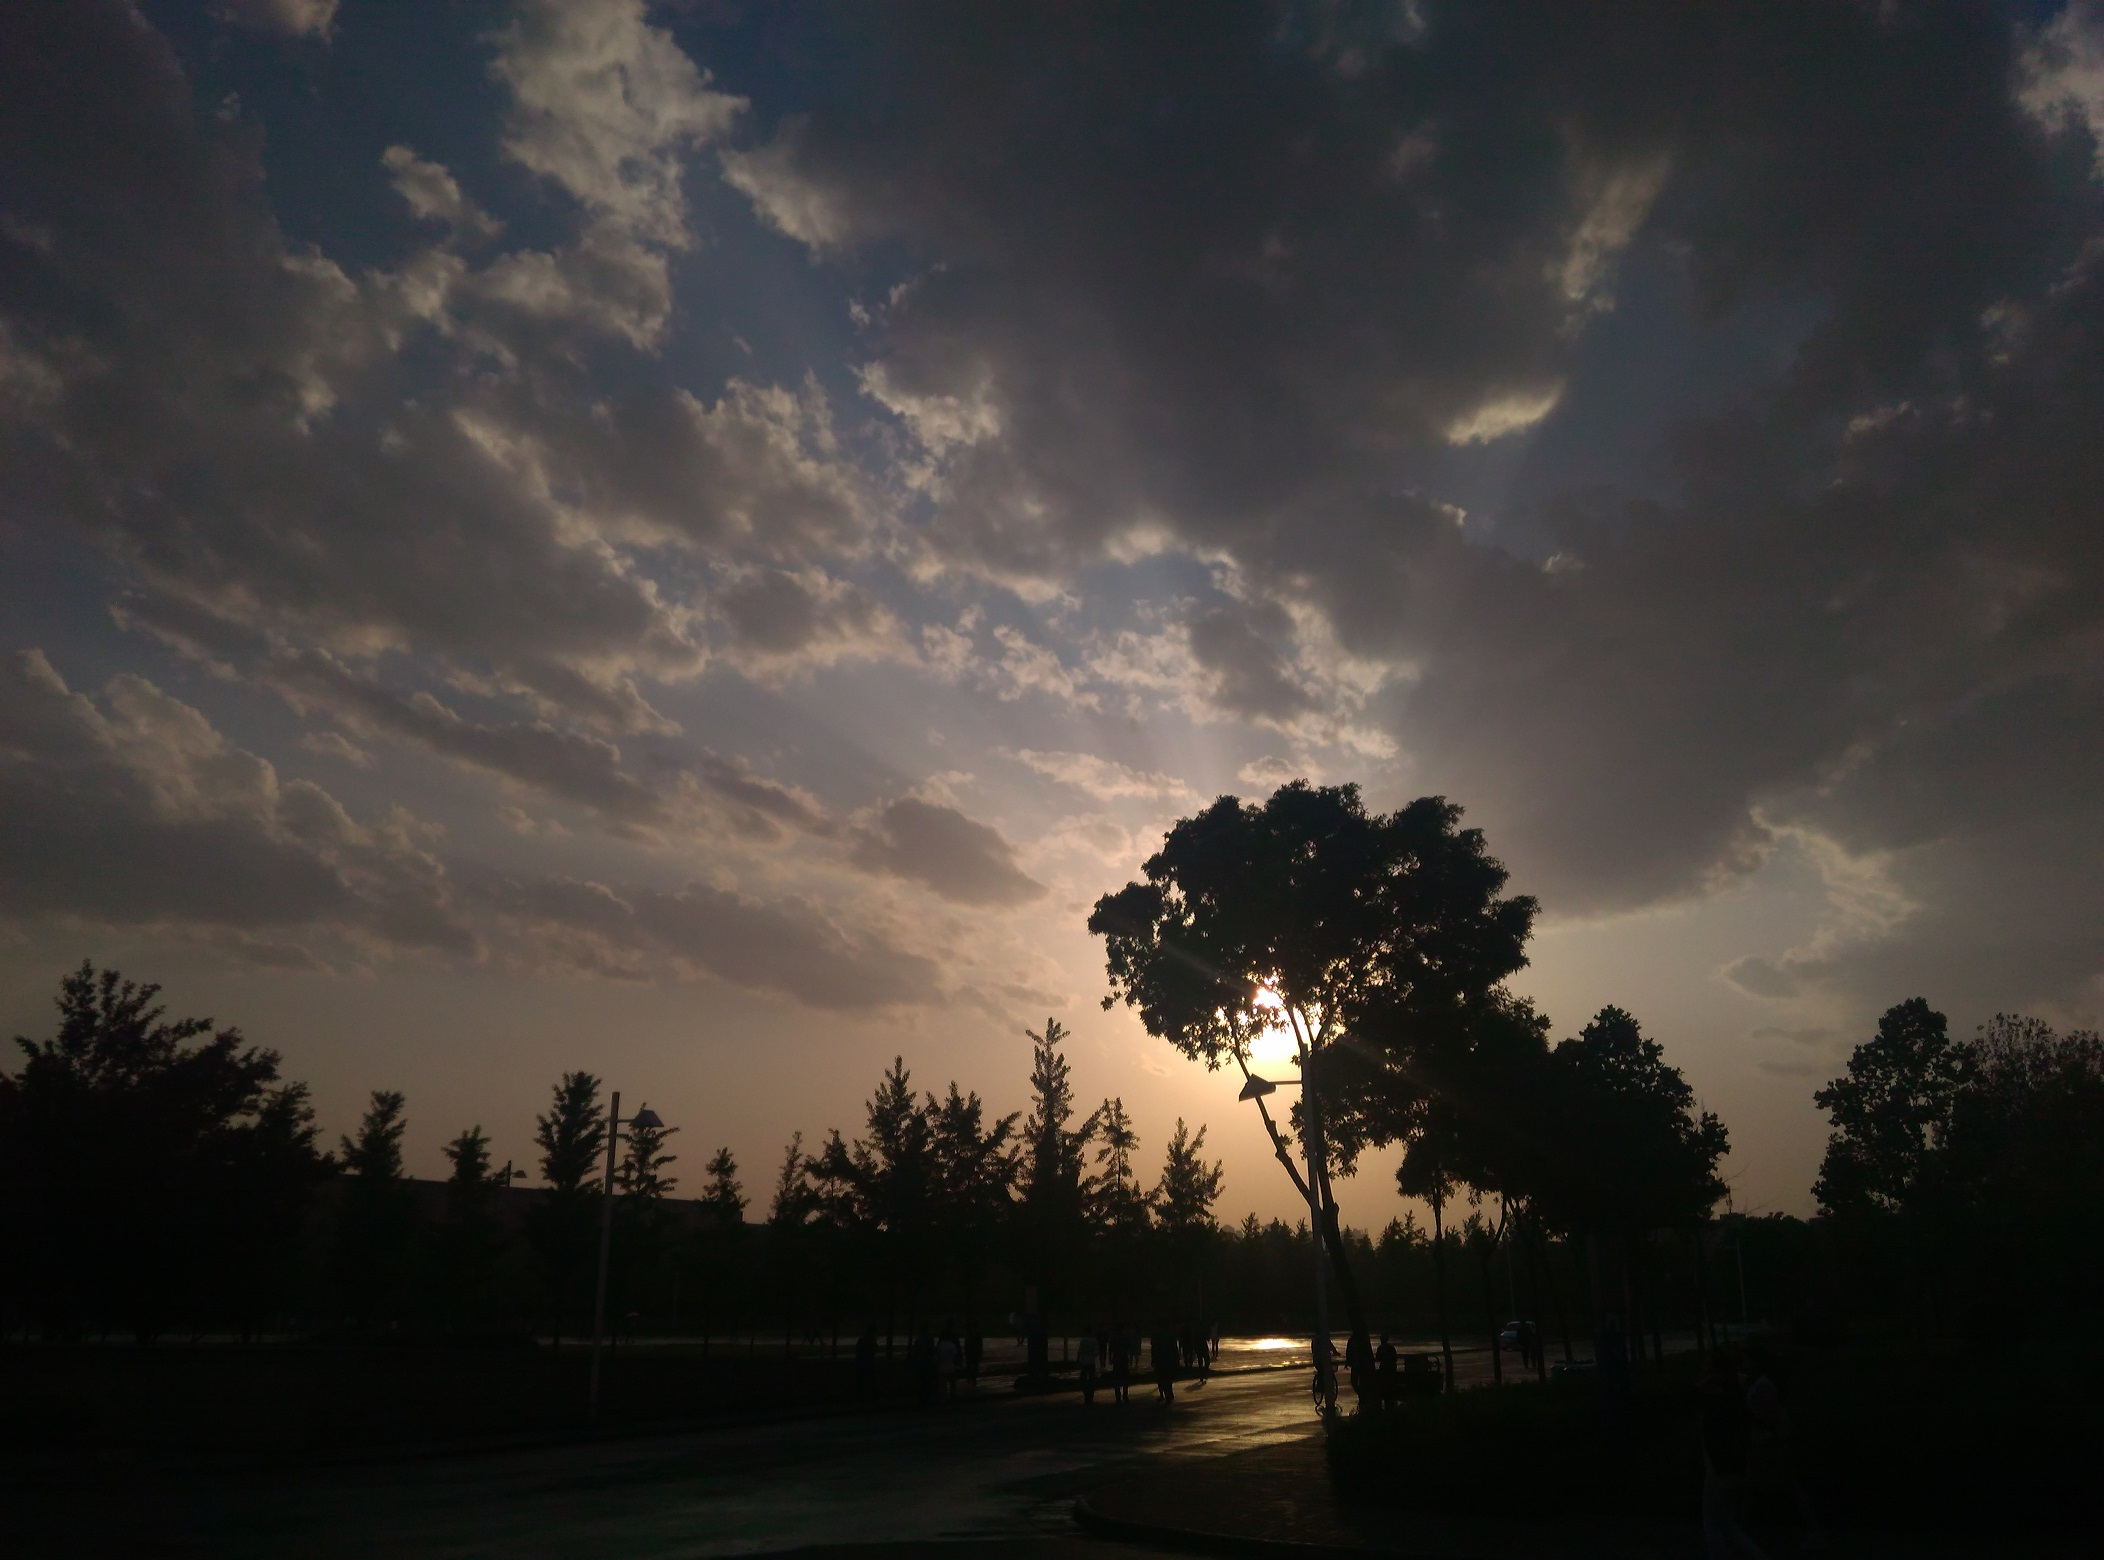
\includegraphics[width=.45\linewidth]{./Figure/IMG_XD4.jpg}}
\subcaptionbox{西电5}
{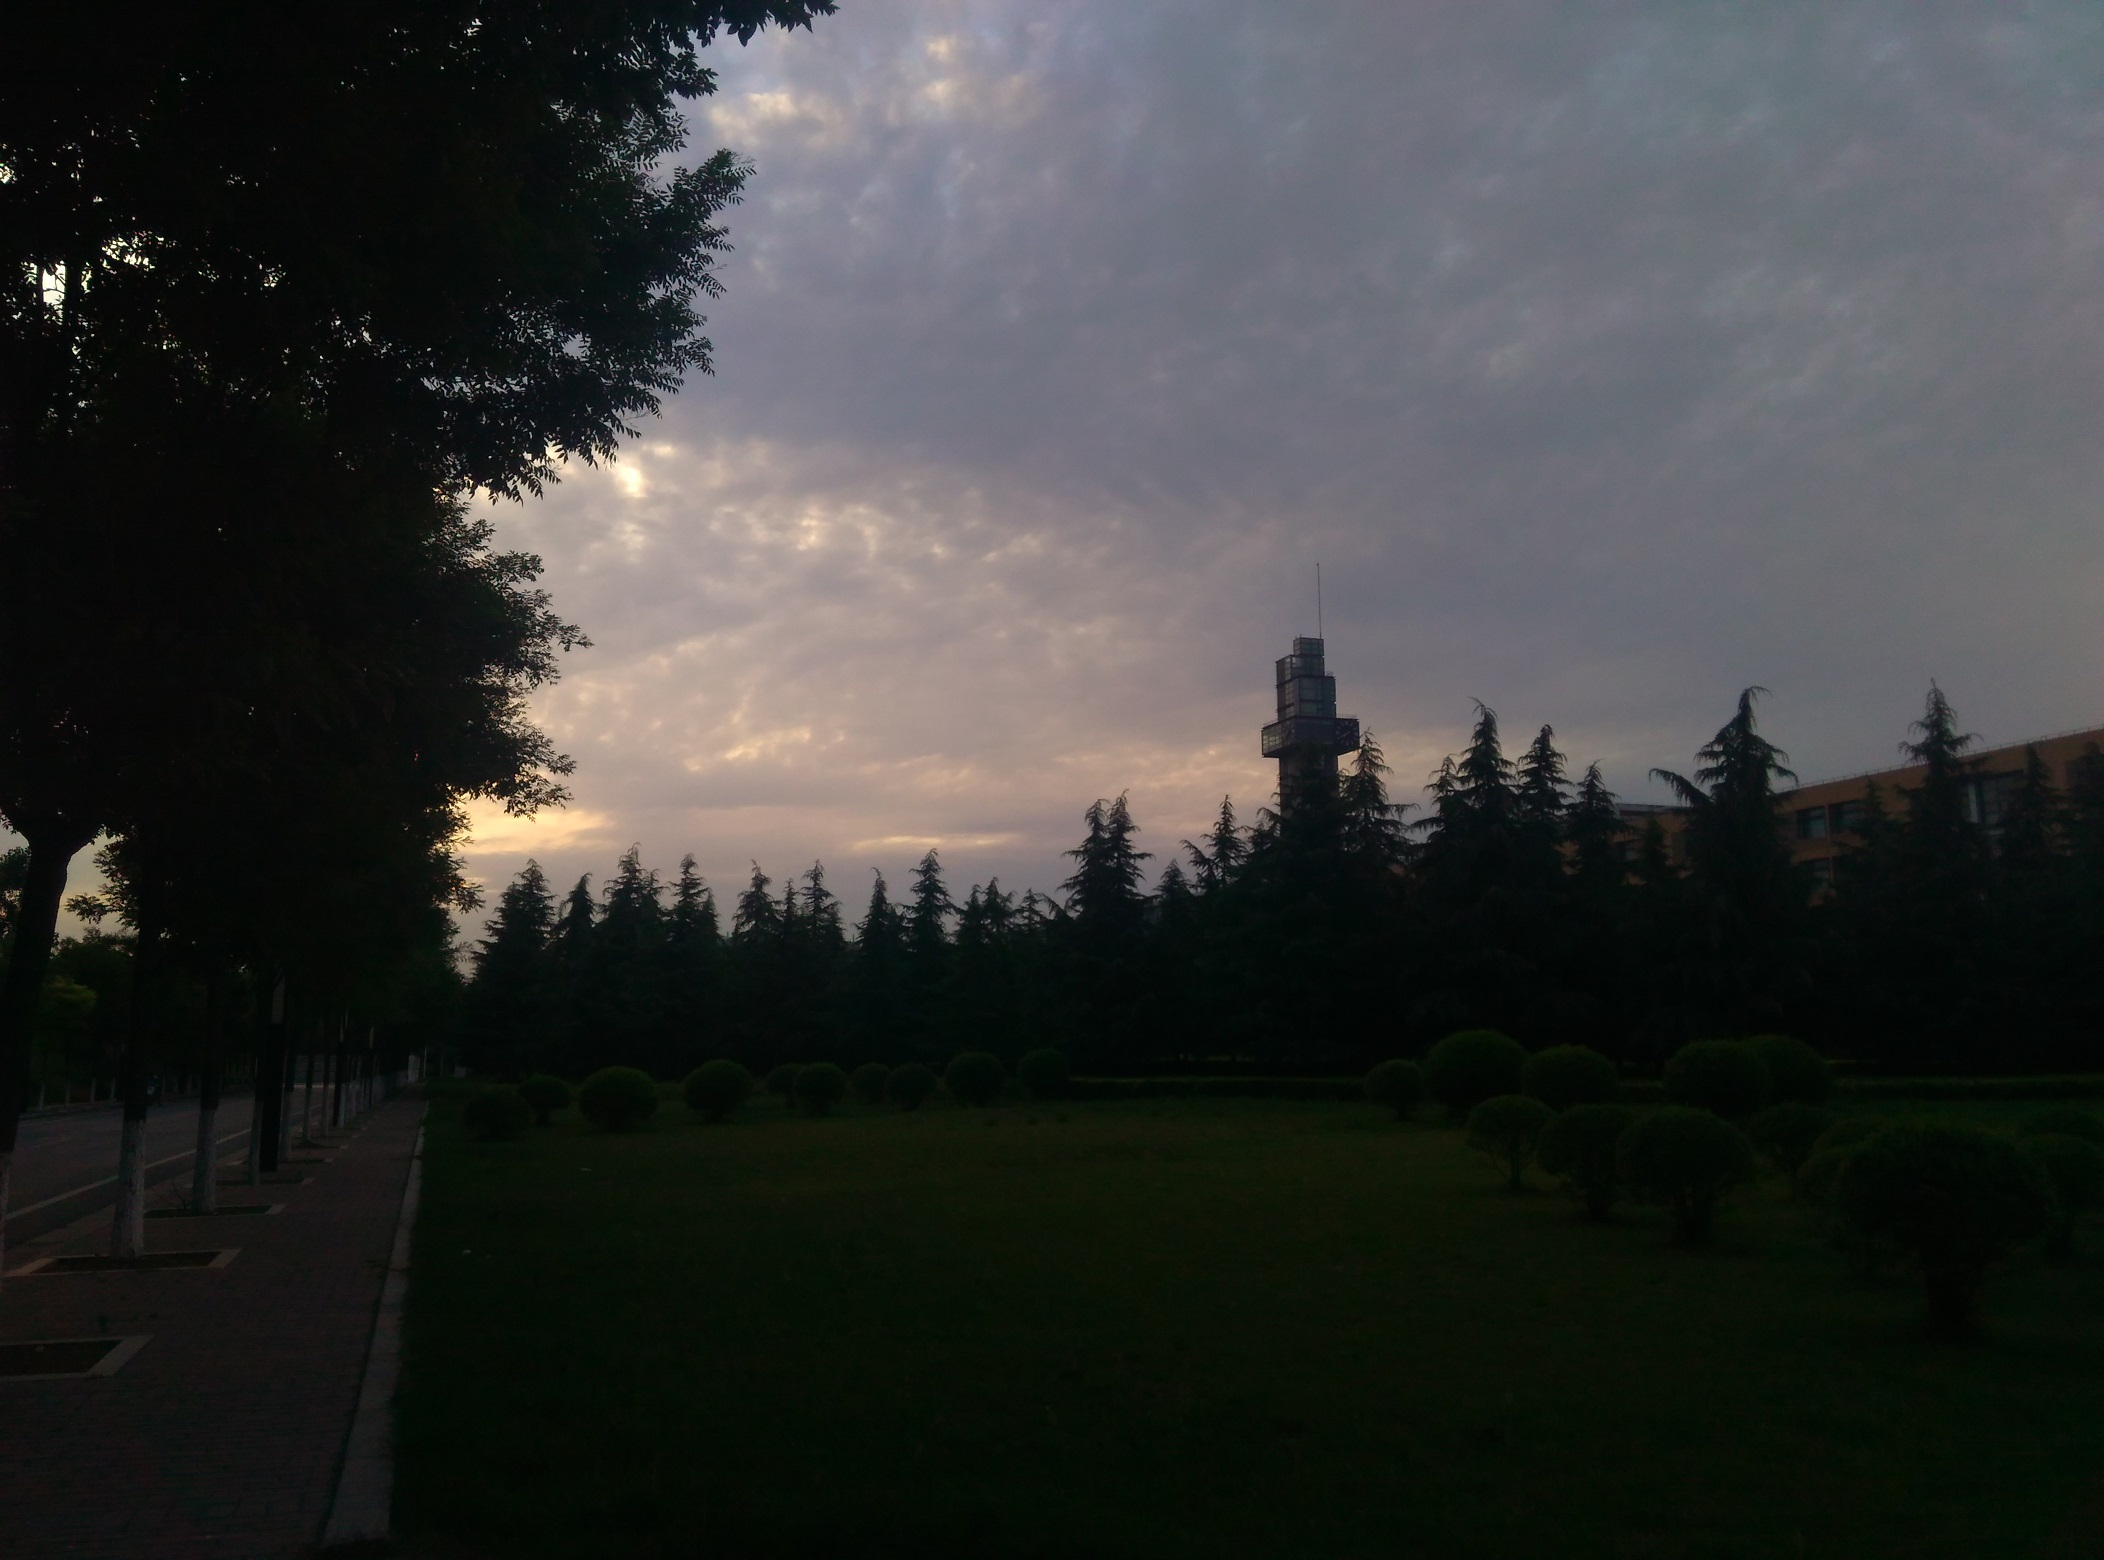
\includegraphics[width=.45\linewidth]{./Figure/IMG_XD5.jpg}}
\caption{并排插图}\label{Fig:bingpai}
\end{figure}

插图就介绍到这,其他知识自学。

\section{公式}
\subsection{普通公式}
先来看一个行内公式:$y=x+1$.

下面是一个居中的公式:
\[
f(X)=\sum_{i=1}^{n}\sin{\frac{\pi}{2}x_i}
\]

看一个编号的公式,如式\eqref{Eq:eq1}:
\begin{equation}\label{Eq:eq1}
f(X)=\sum_{i=1}^{n}\sin{\frac{\pi}{2}x_i}
\end{equation}

\subsection{复杂公式}
\begin{itemize}
\item \textbf{多行公式}

\begin{equation}\label{Eq:eq2}
\begin{aligned}
f(x) &= \sin(a+b)\\
&= \sin(a)\cos(b)+\cos(a)\sin(b).
\end{aligned}
\end{equation}

\begin{equation}\label{Eq:eq3}
f(x) = \left\{
\begin{aligned}
 -&x+1,\quad \text{if}~x<0;\\
 &x+1,\quad \text{if}~x \geq 0;
 \end{aligned}
 \right.
\end{equation}

\item \textbf{矩阵}

\[
  A = \left(\begin{array}{ccc}
        a_{11} & a_{12} & a_{13} \\
        a_{21} & a_{22} & a_{23} \\
        a_{31} & a_{32} & a_{33}
      \end{array}\right),\quad
  B = \left[\begin{array}{ccc}
        b_{11} & b_{12} & b_{13} \\
        b_{21} & b_{22} & b_{23} \\
        b_{31} & b_{32} & b_{33}
      \end{array}\right],\quad
   C = \left[\begin{array}{ccc}
     c_{11} & c_{12} & c_{13} \\
     \vdots & \ddots & \vdots \\
     c_{31} & c_{32} & c_{33}
   \end{array}\right].
\]
行列式也类似
\[
A = \left|\begin{array}{ccc}
    a_{11} & a_{12} & a_{13} \\
    a_{21} & a_{22} & a_{23} \\
    a_{31} & a_{32} & a_{33}
  \end{array}\right|.
\]

\item \textbf{其他公式}

\[
\mathbb{L} = \int_{x_1}^{x_2}\sqrt{1+(y')^2}dx 
= \frac{1}{\alpha}\int_{x_1}^{x_2}y''(x)dx
\]

\end{itemize}

\section{休息一下}

\subsection{山水之间}
\begin{center}
\textbf{山水之间}

{\kaishu 许嵩}

\vspace*{1em}
昨夜同门云集\quad 推杯又换盏\\
今朝茶凉酒寒\quad 豪言成笑谈\\
半生累\quad 尽徒然\\
碑文完美有谁看\\
隐居山水之间\quad 誓与浮名散\\

\vspace*{.6em}
湖畔青石板上\quad 一把油纸伞\\
旅人停步折花\quad 淋湿了绸缎\\
满树玉瓣多傲然\\
江南烟雨却痴缠\\
花飞雨追\quad 一如尘缘理还乱\\

\vspace*{.6em}
落花雨\quad 你飘摇的美丽\\
花香氤\quad 把往日情勾起\\
我愿意\quad 化浮萍躺湖心\\
只陪你\quad 泛岁月的涟漪
\end{center}

\subsection{念奴娇·赤壁怀古}

\begin{center}
\textbf{念奴娇·赤壁怀古}

{\kaishu 苏轼}

\vspace*{1em}
大江东去,浪淘尽,千古风流人物。\\
故垒西边,人道是:三国周郎赤壁。\\
乱石穿空,惊涛拍岸,卷起千堆雪。\\
江山如画,一时多少豪杰。\\

\vspace*{.8em}
遥想公瑾当年,小乔初嫁了,雄姿英发。\\
羽扇纶巾,谈笑间樯橹灰飞烟灭。\\
故国神游,多情应笑我,早生华发。\\
人生如梦,一尊还酹江月。

\end{center}

这一章就写到这里吧,下一章重点介绍两个内容

\chapter{两个重点}
这一章,会涉及到环境以及参考文献两个重点东西。

\section{环境}
\subsection{定理类环境}

\begin{proposition}\label{prop:p1}
这是一个命题。
\end{proposition}

它还可以这么写,所有定理类环境,都可这么写。

\begin{proposition}[命题名]
由命题 \ref{prop:p1}, 这也是一个命题。
\end{proposition}

\begin{assumption}
距离水平面$100\,m$以内,重力加速度$g$是不变的。
\end{assumption}

\begin{lemma}[法图引理]
设$(S,\Sigma,\mu)$为一个测度空间,$(f_n)_{n\geq 0}$是一个实值的可\textbf{正值}函数列。那么:
\[
\int_S \liminf_{n\rightarrow \infty} f_n d\mu \leqslant \liminf_{n\rightarrow \infty} \int_S f_n d\mu.
\]
其中函数极限是在逐点收敛的意义上的极限,函数取值和积分可以是无限大的。
\end{lemma}

\begin{theorem}
若$\lim_{n\rightarrow \infty} x_n = a$,则$\{x_n\}$的任何子列$\{x_{n_k}\}$都收敛于$a$.
\end{theorem}
\begin{proof}
因$\lim_{n\rightarrow \infty} x_n = a$,对任意给定的$\varepsilon > 0$,必定存在正整数$N$,当$n>N$时,有
\[
|x_n-a|<\varepsilon.
\]
今取$K=N$,则对一切$k>K$,有$n_k>n_K=n_N\geq N$,这时就有
\[
|x_{n_k} - a|<\varepsilon.
\]
\end{proof}

\subsection{代码环境}

\begin{lstlisting}[language=C]
#include<stdio.h>

int main()
{
	printf("Hello World!");
	return 0;
}
\end{lstlisting}

\begin{lstlisting}[language=C,caption={Java代码},label=Code:java]
package com.stick.test;

/**
 * 公共主类;
 * 类名必须与文件名相同
 */
public class Test{
	public static void main(String[] args) {
		System.out.println("Hello World!");
	}
}
\end{lstlisting}

\begin{lstlisting}[language=R,style = nonumbers]
x<-c(1,2,3,4,5,6)
y<-sin(x)
lines(x,y)
\end{lstlisting}
\section{参考文献的引用}
以下为常用的参考文献。

期刊\cite{Art,ArtE},专著(无页码)\cite{Boo,BooE,Boo1},专著(含页码)\cite{InBoo,InBoo1,InBooE},论文集\cite{Incol,IncolE}。

硕士\cite{MT}/博士论文\cite{Phd},科技报告\cite{TechR}。

以下参考文献,原有plain风格中并无,为Stick本人自己写的。

网络内容引用\cite{Net},译著\cite{Trans}

此外,多说一句,本文模板加载的 \verb=natbib= 宏包使得 \verb=\cite= 命令还支持排序等功能。

比如下列文献\cite{ArtE,BooE,InBooE,Trans,Net}